\documentclass[11pt]{article}
\usepackage{geometry}
\geometry{a4paper, top=20mm, left=10mm, right=10mm, bottom=20mm}
\usepackage{graphicx}
\usepackage{amsmath,amssymb,amsthm}
\usepackage{amssymb}
\usepackage[utf8]{inputenc}
\usepackage{fancyhdr}
\usepackage{lastpage}
\usepackage{enumerate}
\usepackage{enumitem}
\usepackage{tikz}
\usetikzlibrary{shapes.geometric}
\usepackage{multicol}
\usepackage{subcaption}
\usepackage{ifthen}
%------------------------------------------ preamble
%----- fancyhdr
\fancyhead[R]{Übungsgruppe: 2 (Do 12-14)}
\fancyhead[C]{Name: Maurice Wenig}
\fancyhead[L]{Matrikelnummer: 178049}
\fancyfoot{}
\rfoot{Seite \thepage\ von \pageref{LastPage}}
\pagestyle{fancy}
%----- aufgaben
\newtheoremstyle{break}{}{5mm}{}{}{\bfseries}{}{0mm}
{\textbf{\thmname{#1}\thmnumber{ #2:} \thmnote{\textit{#3}}\newline}}
\theoremstyle{break}
\newtheorem{task}{Aufgabe}
%----- new commands
\newcommand{\Romannumeral}[1]{\MakeUppercase{\romannumeral #1}}
%----- tikz automata
\usetikzlibrary{arrows, automata, positioning}
%------------------------------------------ main
\begin{document}
%----- title
\begin{center}
\Large{Automaten und Berechenbarkeit}\\
\large{2. Übungsserie}
\end{center}
%----- tasks
\begin{task}
\hfill\vspace{-5mm}
\begin{enumerate}[label={(\alph*)}]
\item \hfill\vspace{-5mm}\\
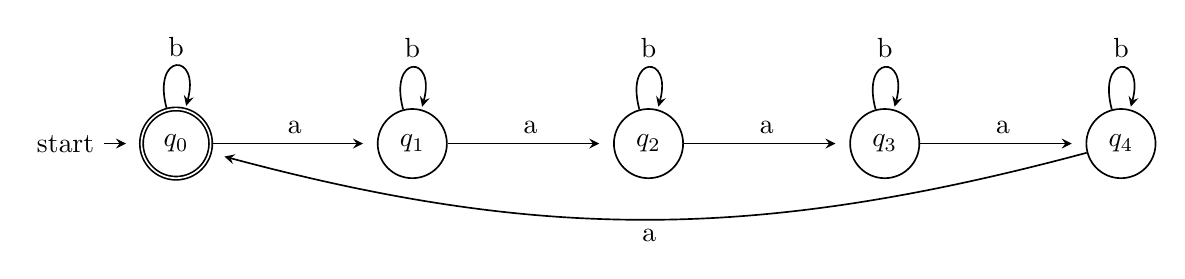
\begin{tikzpicture}[->, > = stealth, shorten > = 5 pt, node distance = 3cm, semithick]

\node[state, initial, accepting]		(0)						{$q_0$};
\node[state]							(1) [right of=0]			{$q_1$};
\node[state]							(2) [right of=1] 		{$q_2$};
\node[state]							(3) [right of=2] 		{$q_3$};
\node[state]							(4) [right of=3] 		{$q_4$};

\path	(0)	edge[above]					node {a}			(1);
\path	(0)	edge[above, loop above]		node {b}			(0);
\path	(1)	edge[above]					node {a}			(2);
\path	(1)	edge[above, loop above]		node {b}			(1);
\path	(2)	edge[above]					node {a}			(3);
\path	(2)	edge[above, loop above]		node {b}			(2);
\path	(3)	edge[above]					node {a}			(4);
\path	(3)	edge[above, loop above]		node {b}			(3);
\path	(4)	edge[below, bend left=15]	node {a}			(0);
\path	(4)	edge[above, loop above]		node {b}			(4);

\end{tikzpicture}


\item \hfill\vspace{-5mm}\\
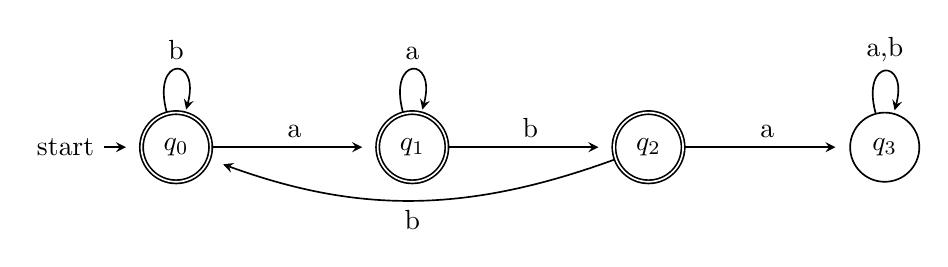
\begin{tikzpicture}[->, > = stealth, shorten > = 5 pt, node distance = 3cm, semithick]

\node[state, initial, accepting]		(0)						{$q_0$};
\node[state, accepting]				(1) [right of=0]			{$q_1$};
\node[state, accepting]				(2) [right of=1] 		{$q_2$};
\node[state]							(3) [right of=2] 		{$q_3$};

\path	(0)	edge[above]					node {a}			(1);
\path	(0)	edge[above, loop above]		node {b}			(0);
\path	(1)	edge[above]					node {b}			(2);
\path	(1)	edge[above, loop above]		node {a}			(1);
\path	(2)	edge[above]					node {a}			(3);
\path	(2)	edge[below, bend left=20]	node {b}			(0);
\path	(3)	edge[above, loop above]		node {a,b}		(3);

\end{tikzpicture}


\item \hfill\vspace{-5mm}\\
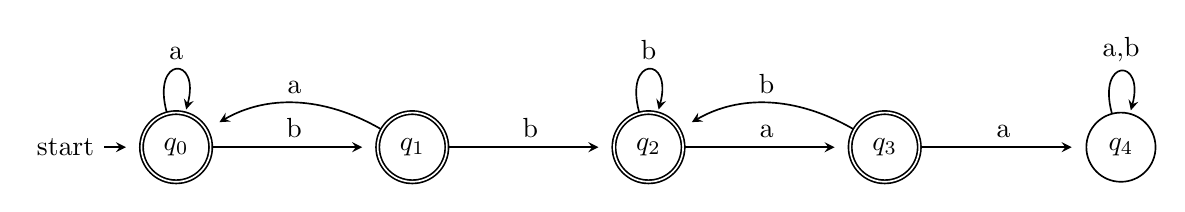
\begin{tikzpicture}[->, > = stealth, shorten > = 5 pt, node distance = 3cm, semithick]

\node[state, initial, accepting]		(0)						{$q_0$};
\node[state, accepting]				(1) [right of=0]			{$q_1$};
\node[state, accepting]				(2) [right of=1] 		{$q_2$};
\node[state, accepting]				(3) [right of=2] 		{$q_3$};
\node[state]							(4) [right of=3] 		{$q_4$};

\path	(0)	edge[above]					node {b}			(1);
\path	(0)	edge[above, loop above]		node {a}			(0);
\path	(1)	edge[above, bend right]		node {a}			(0);
\path	(1)	edge[above]					node {b}			(2);
\path	(2)	edge[above]					node {a}			(3);
\path	(2)	edge[above, loop above]		node {b}			(2);
\path	(3)	edge[above]					node {a}			(4);
\path	(3)	edge[above, bend right]		node {b}			(2);
\path	(4)	edge[above, loop above]		node {a,b}			(4);

\end{tikzpicture}
\end{enumerate}
\end{task}

\begin{task}
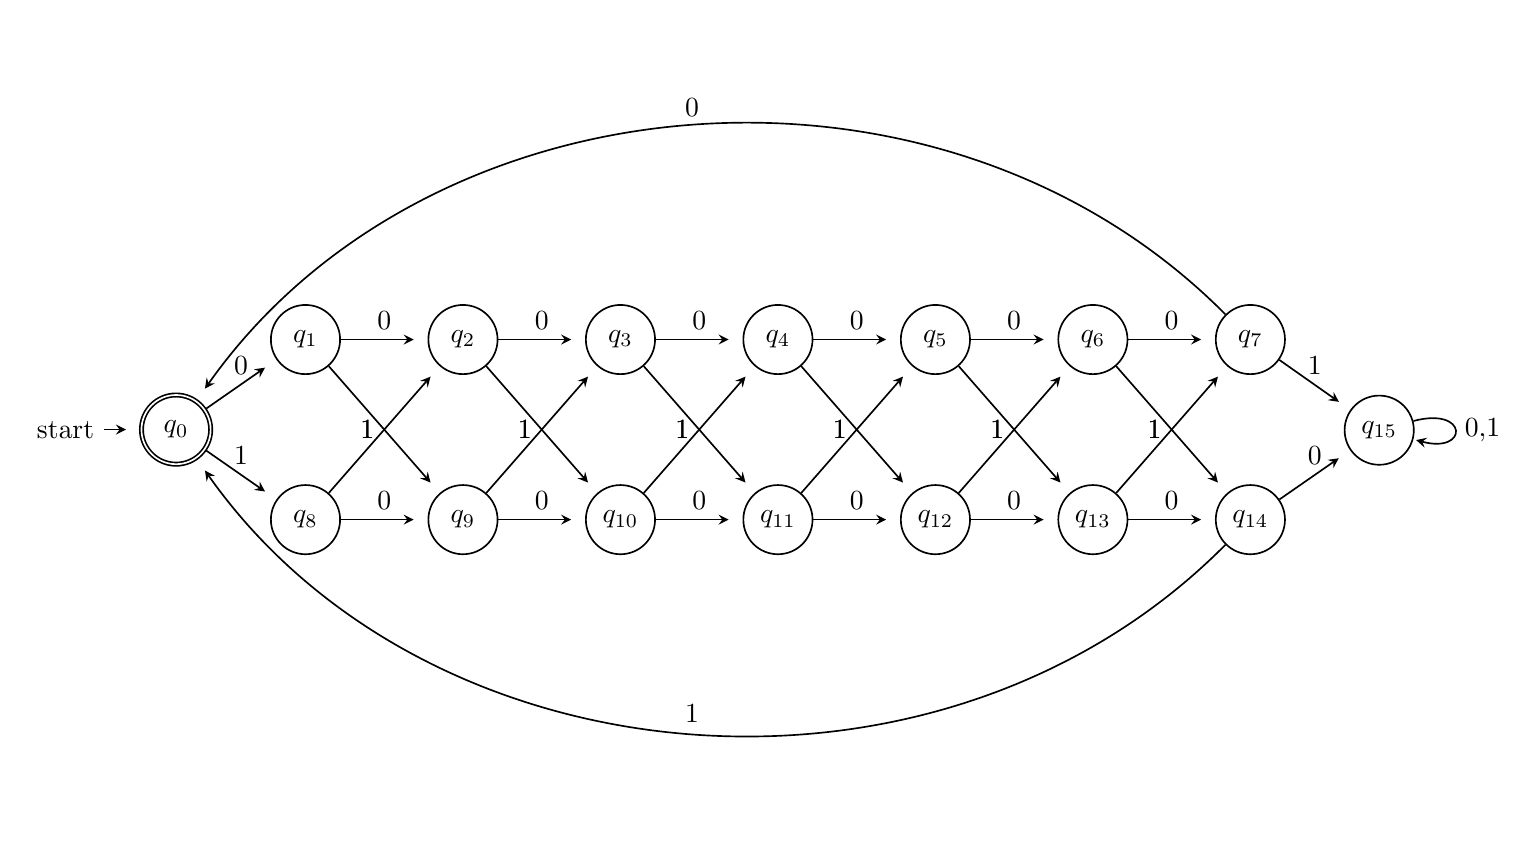
\begin{tikzpicture}[->, > = stealth, shorten > = 5 pt, node distance = 2cm, semithick]

\node[state, initial, accepting]		(0)						{$q_0$};
\node[state]							(1) [above right=5mm and 10mm of 0]	{$q_1$};
\node[state]							(2) [right of=1] 		{$q_2$};
\node[state]							(3) [right of=2] 		{$q_3$};
\node[state]							(4) [right of=3] 		{$q_4$};
\node[state]							(5) [right of=4] 		{$q_5$};
\node[state]							(6) [right of=5] 		{$q_6$};
\node[state]							(7) [right of=6] 		{$q_7$};

\node[state]							(8) [below right=5mm and 10mm of 0]	{$q_{8}$};
\node[state]							(9) [right of=8] 		{$q_{9}$};
\node[state]							(10) [right of=9] 		{$q_{10}$};
\node[state]							(11) [right of=10] 		{$q_{11}$};
\node[state]							(12) [right of=11] 		{$q_{12}$};
\node[state]							(13) [right of=12] 		{$q_{13}$};
\node[state]							(14) [right of=13] 		{$q_{14}$};
\node[state]							(15) [above right=5mm and 10mm of 14]	{$q_{15}$};


\path	(0)	edge[above]					node {0}			(1);
\path	(1)	edge[above]					node {0}			(2);
\path	(2)	edge[above]					node {0}			(3);
\path	(3)	edge[above]					node {0}			(4);
\path	(4)	edge[above]					node {0}			(5);
\path	(5)	edge[above]					node {0}			(6);
\path	(6)	edge[above]					node {0}			(7);

\path	(0)	edge[above]					node {1}			(8);
\path	(8)	edge[above]					node {0}			(9);
\path	(9)	edge[above]					node {0}			(10);
\path	(10)	edge[above]					node {0}			(11);
\path	(11)	edge[above]					node {0}			(12);
\path	(12)	edge[above]					node {0}			(13);
\path	(13)	edge[above]					node {0}			(14);

\path	(1)	edge[left]					node {1}			(9);
\path	(2)	edge[left]					node {1}			(10);
\path	(3)	edge[left]					node {1}			(11);
\path	(4)	edge[left]					node {1}			(12);
\path	(5)	edge[left]					node {1}			(13);
\path	(6)	edge[left]					node {1}			(14);
\path	(7)	edge[above]					node {1}			(15);

\path	(8)	edge[left]					node {1}			(2);
\path	(9)	edge[left]					node {1}			(3);
\path	(10)	edge[left]					node {1}			(4);
\path	(11)	edge[left]					node {1}			(5);
\path	(12)	edge[left]					node {1}			(6);
\path	(13)	edge[left]					node {1}			(7);
\path	(14)	edge[above]					node {0}			(15);

\path	(7)	edge[above, bend right=50]	node {0}			(0);
\path	(14)	edge[above, bend left=50]	node {1}			(0);
\path	(15)	edge[right, loop right]		node {0,1}		(15);

\end{tikzpicture}
\end{task}
\newpage
\begin{task}
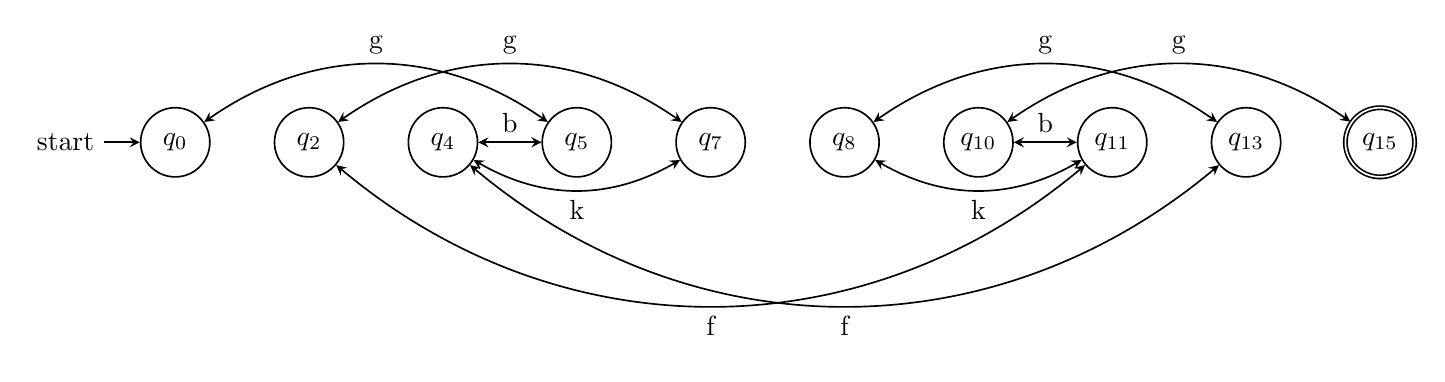
\begin{tikzpicture}[->, > = stealth, node distance = 1.7cm, semithick]

\node[state, initial]				(0)						{$q_{0}$};
\node[state]							(2) [right of=0]			{$q_{2}$};
\node[state]							(4) [right of=2] 		{$q_{4}$};
\node[state]							(5) [right of=4] 		{$q_{5}$};
\node[state]							(7) [right of=5] 		{$q_{7}$};
\node[state]							(8) [right of=7] 		{$q_{8}$};
\node[state]							(10) [right of=8] 		{$q_{10}$};
\node[state]							(11) [right of=10] 		{$q_{11}$};
\node[state]							(13) [right of=11] 		{$q_{13}$};
\node[state, accepting]				(15) [right of=13] 		{$q_{15}$};

\path	(4)	edge[<->, above]					node {b}			(5);
\path	(10)	edge[<->, above]					node {b}			(11);
\path	(4)	edge[<->, below, bend right]		node {k}			(7);
\path	(8)	edge[<->, below, bend right]		node {k}			(11);
\path	(0)	edge[<->, above, bend left=35]		node {g}			(5);
\path	(2)	edge[<->, above, bend left=35]		node {g}			(7);
\path	(8)	edge[<->, above, bend left=35]		node {g}			(13);
\path	(10)	edge[<->, above, bend left=35]		node {g}			(15);
\path	(2)	edge[<->, below, bend right=40]	node {f}			(11);
\path	(4)	edge[<->, below, bend right=40]	node {f}			(13);
\end{tikzpicture}\\
Alle nicht dargestellten Kanten führen auf einen Mülleimer. (ohne Mülleimer besser lesbar)
\end{task}
\end{document}
